\subsection{Motivation} Motivation of the model we studied can be found in the
IP-based computer networks problems. Router has to store enormous number of
forwarding rules and this number is still growing. The fast router memory is
expensive and requires a lot of energy, which is a big problem for Internet
Service Providers. As a solution to this problem there comes Software-Defined
Networking (SDN) technology. It consists of two types of memory: the fast
memory, which is kept in router and the slow one, which is placed in so called
controller. The latter one keeps exact information about all of the FIB rules.
On the other hand, router keeps only the part of the FIB tree. Whenever a packet
comes, it is firstly processed by the router. If its forwarding rule is found in
the router's cache, then it is immediately forwarded to its final destination.
In the case of not finding the appropriate rule for the packet, we have to ask
the controller, therefore look up the rule in the slow memory paying $1$ for
each such request. The routers cache can change its state, but it might be
expansive. Precisely, if we decide to erase a single rule form the router or
fetch it form the controller to the router, we pay $\alpha$ for each such
opertion.  Moreover, occasionaly there might occure an update on some rule in
controller's FIB table.  If the corresponting rule is in the router, we are
obligated to update it immediately, what cost us $\alpha$ as well. Figure
\ref{fig:motivation} shows the crucial concepts, that were just briefly
described. More detailed and technical description can found in \cite{sdn}.
\begin{figure} \begin{center}
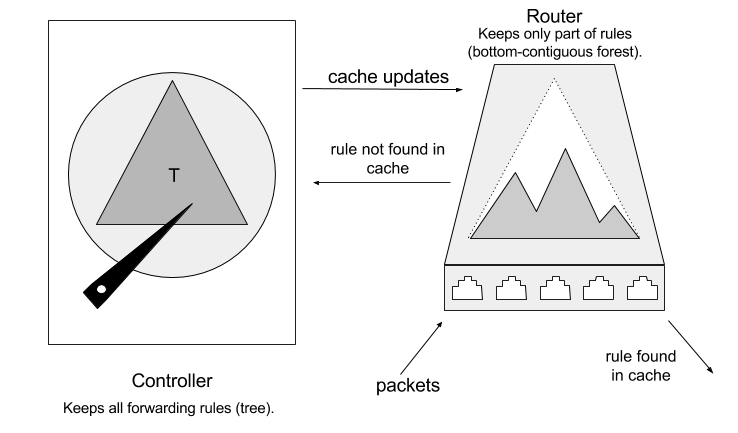
\includegraphics[width=0.8\textwidth]{motivation.png} \end{center} \caption{}
\label{fig:motivation} \end{figure}

Since the rules are taken from forwarding table, what we look for is the rule
with the longest matching prefix (LMP). Whenever a packet arrives, the router
will look for the rule which matches the longest prefix of destination IP
address of that packet. So the search can be viewed as going down the tree,
whose nodes preserve information of IP address prefix, its root keeps the least
specific (empty) rule, and descendants of node representing IP prefix $p$ are
the nodes with rules $p \circ x$ where operation $\circ$ is concatenation of
binary representations of $p$ and $x$. The deeper in the tree we can go, the
more specific rule we find. We add special rule, which is kept in the root of
routers cache tree, that matches every prefix and points to the controller. It
solves the problem of when we decide to ask controller when any rule can't be
found in the routers cache. Note, that besides the tree like structure, that we
now see the routers cache consists of, there is natural requirement of the
rooter tree to be bottom-contiguous. Otherwise we would not in some cases find
the most specific rule and therefore forward the packet to the wrong address. 

Summing up, we can define a model for SDN architecture, which from now on will
be called SDN model. In that model, as in the tree caching model, we have a tree
$T$, whose nodes are requested, fast memory (cache) that can store $\kind{ONL}$
elements (which are rules) which form a bottom-contiguous forest and the slow
memory keeping the whole tree structure. The input consists of requests to the
elements of the tree - cached iteams we serve for free finding the approprate
rule in cahce, whereas the ones that much only special rule (empty) requires
asking the controller and thus we pay $1$. Any change in the cache cost us
$\alpha$, so the same as in the tree caching model. We have additional event
though. Whenever controller rule is updated, we update the corresponding rule in
the routers cache paying $\alpha$ if it is present in the routers cache,
otherwise we do not update and do not have to pay anything.

Now we will use an algorithm $TC$ solving the tree caching problem as a black
box and use it to solve the SDN setting (by defining algorithm $ALG$ based on
$TC$). First, the tree from the SDN model is mapped to the tree caching model's
tree using identity function. Let $\sigma$ be the input for the SDN model. We
transform it to $\sigma'$, which will be the input for $TC$. We do so by adding
$\alpha$ negative requests to the rule at every time when it was updated in the
controller (recall, that in the SDN model in such situation we are obtaining
cost $\alpha$ for the update if the rule was in cache). The rest of the input
stays the same with the exception, that all these requests are positive. Now
$ALG$ is defined such a way, that given input sequence $\sigma$ it copies the
moves (fetches and evictions) of $TC$ given modified input $\sigma'$. The
following theorem states, that using such application of $TC$, we can get the
same competitive ratio algorithm for the SDN model as for the tree caching model
up to the constant factor. Therefore, solving the tree caching problem gives as
competitive algorithm for the SDN model, so finds a very usefull practical
application.  
\begin{theorem} 
Let $TC$ be any algorithm solving the tree caching
problem, that is $r$-competitive. Let $ALG$, $\sigma$ and $\sigma'$ be defined
as above with respect to $TC$. Then: $$cost_{\mathrm{ALG}}(\sigma) \leq c \cdot
cost_{\mathrm{TC}}(\sigma') \leq c \cdot r \cdot cost_{\mathrm{OPT'}}(\sigma')
\leq c \cdot r \cdot cost_{\mathrm{OPT}}(\sigma),$$ where $c$ is a constant and
$cost_{\mathrm{OPT'}}(\sigma')$ relates to the cost on the input $\sigma'$ of
optimal offline solution in the tree caching model and the
$cost_{\mathrm{OPT}}(\sigma)$ relates to cost of optimal offline solution on the
input $\sigma$ for the SDN model. In other words, $ALG$ has the same competitive
ratio
as $TC$ up to the constant factor. 
\end{theorem} 
\begin{proof}
The second inequality we have from definition of $TC$ being $r$-competitive. To
prove the first inequality we have to compare the costs of $ALG$ on $\sigma$
with the cost of $TC$ on $\sigma'$. Let $f$
be the mapping from request from $\sigma$ to the positive requests of $\sigma'$
preserving the chronology of events. For any update $u$ to rule in the
controller we assign $m(u)$, which is a set of $\alpha$ negative requests that this
update made to be added to $\sigma'$. There are three cases when $ALG$ has to pay.
\begin{enumerate}
\item $ALG$ process the request $\sigma_t$ to element, that is not present in
$ALG$'s cache. Then
it pays $1$ for it. $TC$ has the same cache state when it processes the corresponding
positive request $f(\sigma_t)$ paying $1$ as well.
\item $ALG$ makes a reorganization of the cache. Recall, it makes the same
reorganizations as $TC$, thus the overall cost related to changing the cache is
the same for both algorithms.
\item Update $u$ takes place for some rule in the controller, so $ALG$ pays $\alpha$.
The same time we have sequence of $\alpha$ negative requests to $m(u)$. $ALG$
pays then at least $\alpha$ on that sequence - either for all the requests or the
cache update.
$ALG$ and $TC$ both does not pay for any other requests or events. Cost originating
from updates for $ALG$ were counted at most twice (look at the two last points
above), therefore $cost_{ALG}(\sigma) \leq 2 \cdot cost_{TC}(\sigma')$, which
ends the proof of first in equality.

Now we proceed to the proof of the last inequality. Consider the following
offline algorithm $OFF$ for the tree caching problem. It makes the same moves as
the $OPT$ on $\sigma$. It does not pays on updates what compensates the cost
occured on the negative requests, so $cost_{OFF}(\sigma') \leq
cost_{OPT}(\sigma)$. Obviously, $cost_{OPT'}(\sigma') \leq cost_{OFF}(\sigma')$,
what ends the proof.
\end{enumerate}
\end{proof}
